%\subsection{Incremental facility location}
%\label{sec:incremental}

\red{details of static version here}

\subsection*{Algorithm for the \probinc{} problem}
In this section, we consider the setting where facilities might be deployed incrementally, with a fixed capacity. We consider a given schedule $t_0, t_1, \ldots, t_m$, which denote the discrete times at which we want to monitor the epidemic. At time $t_u$, we let $k_u \geq 0$ denote the number of new facilities with uniform capacity $cap_u \geq 1$ that can be deployed. We also $\mathbf{p}(t_u)$ be the demand vector at time $t_u$. In our experiments, $t_1, t_2, \ldots, t_m$ are equidistant and corresponding to the times after $1$ week, $2$ weeks, and so on. Our method \textsc{OnlineKMed} starts with an initial
deployment of $k_0$ facilities at time $t_0$, based on the population density, and at each subsequent time $t_u$ with $u > 0$, it uses the current infection rates to determine the locations where $k_u$ additional facilities could be deployed, \emph{without altering the locations of facilities already deployed}. Let $O_u$ denote the set of open hospital at time $t_u$. We require that $O_0 \subseteq O_1 \subseteq O_2 \ldots \subseteq O_m$.

Let us consider any time $t_u$ where $u > 0$. Let $C_{u-1}$ denote the total capacities of all hospital up to time $t_{u-1}$. The first question is ``how should we determine the number $k_u$ of new hospitals to be built?'' In practice, there are two main factors for estimating parameter $k_u$: (1) our current budget and (2) the forecasted demand vectors $\mathbf{p}(t_v)$ for a few next time points $\{t_v: v \geq u\}$. Indeed we want to cover as many population nodes as possible; however, the total opening cost will have to be bounded by some given budget.

Now suppose we know the value of $k_u$. Then the maximum number of patients who can be served is $C_u = C_{u-1} + k_u \times cap_u$. We have two cases:
\begin{itemize}
	\item Case $C_u \geq |\mathbf{p}(t_u)|_1$: it is possible to serve all patients at time $t_u$. We solve the corresponding capacitated $k$-median instance with the set $O_{u-1}$ being opened and obtain the solution $O_u$. Now the optimal assignment of patients to open facilities in $O_u$ can be easily found by solving a minimum cost max-flow problem.
	
	\item Case $C_u < |\mathbf{p}(t_u)|_1$: it is impossible to serve all patients at time $t_u$. We suggest the following policy. We sort all patients (recall that the node $j \in P$ has $p_j(t_u)$ patients at time $t_u$) in decreasing order of distance to the nearest hospital in $H$. Let $S_u$ be the set of the top $|\mathbf{p}(t_u)|_1 - C_u$ patients in this list. We refer to $S_u$ as the set of ``outliers'' at time $t_u$. We shall need some alternative treatment for the people in $S_u$. Then we exclude $S_u$ from $P$ to obtain a new demand vector $\mathbf{p}'(t_u)$ such that $|\mathbf{p}'(t_u)|_1 = C_u$. The problem can now be solved as in the first case.
	
\end{itemize}






%%
%%
%%\subsection{Preliminaries}
%%Here, we review the dependent rounding technique from \cite{srin:level-sets} and the minimum cost max-flow problem.
%%
%%\begin{proposition}[\cite{srin:level-sets}]
%%\label{prop:dep-round}
%%There exists an algorithm {\sc DepRound}($\mathbf{y}$) which takes as input a vector $\mathbf{y} \in [0,1]^n$ where $\sum_{i=1}^n y_i = k$, and in polynomial time outputs a vector $\mathbf{Y} \in \{0,1\}^n$  with the following properties:
%%\begin{enumerate}
%%\item $\Pr[Y_i = 1] = y_i$, for all $i \in [n]$,
%%\item $\sum_{i=1}^n Y_i = k$ with probability one.
%%\end{enumerate}
%%\end{proposition} 
%%
%%Given a directed graph $G = (V, E)$ with capacity $c_e \in \mathbb{R}^+$ and weight $w_e \geq 0$ on each edge $e \in E$, a source $s$, and a sink $t$. Recall that $f$ is a flow iff it satisfies (1) the capacity constraint: $f_e \leq c_e$ for all $e \in E$ and (2) the conservation constraint: $\sum_{u:(u,v)\in E} f_{(u,v)} = \sum_{u:(v,u) \in E} f_{(v,u)}$ for all $u \in V \setminus \{s, t\}$. The minimum cost max-flow problem is to find a maximum flow $f: E \to \mathbb{R}^+$ from $s$ to $t$ such that the total cost $\sum_e w_e f_e$ is as small as possible.  It is well-known that this problem can be solved efficiently by either linear programming or combinatorial algorithms \cite{flow_book, flow_goldberg, Orlin1997}.
%%
%%



Consider any time point $t_u$. Recall that $k = k_u$ is the number of additional hospitals to be built, $O = O_{u-1}$ is the set of open hospitals up to this time, $\mathbf{p}$ and $P$ are the demand vector and population set after excluding the outliers respectively, and $c = cap_u$ is the capacity for all hospitals to be opened at time $t_u$. For each $i \in O$, recall that $cap(i)$ is the (fixed) capacity of hospital $i$ which was chosen when building $i$. The LP relaxation for the capacitated $k$-median problem at time $t_u$ is as follows.

\begin{alignat}{2}  
  \LP_{\CAPKMED}(O, \mathbf{p}, P, c, k): \min  &  \sum_{i \in H}\sum_{j \in P} p_j d_{ij} x_{ij} \nonumber\\
    \text{s.t.} & \sum_{i \in H} x_{ij} = 1    &\qquad& \forall j \in P  \\
                             &  x_{ij} \leq y_i      && \forall i \in H, j \in P \ \\
                             & \sum_{j \in P} x_{ij} \leq cap(i)      && \forall i \in O  \label{cstr:kmed3} \\
                             & \sum_{j \in P} x_{ij} \leq c      && \forall i \in H \setminus O  \label{cstr:kmed4} \\
                             & y_i = 1    && \forall i \in O  \\
                             &  \sum_{i\in H} y_{i} \leq |O|+k_u      &&  \\
                             & x_{ij},  y_i \in [0,1]&& \forall i \in H, j \in P.\nonumber
\end{alignat}
The constraints (\ref{cstr:kmed3}) and (\ref{cstr:kmed4}) make sure that no hospital will serve more patients than its capacity. 

%%Note that solving this LP will only give us  fractional solutions. In this work, we heavily exploit the dependent rounding scheme \textsc{DepRound} for rounding the LP solutions. The idea is to repeat this procedure some $r$ times and choose the best integral solution obtained in the process.
%%
%%\begin{algorithm}[h]
%%\caption{$\textsc{Round}\left( \mathbf{y}, r \right)$}
%%\begin{algorithmic}[1]
%%\STATE $c \gets +\infty, \mathbf{Y} \gets 0$
%%\FOR{$z=1,2,\ldots,r$}
%%	\STATE $\mathbf{Y}' \gets \textsc{DepRound}(\mathbf{y})$
%%	\IF{$c > $ the cost of opening hospitals in $Y'$}
%%		\STATE $\mathbf{Y} \gets \mathbf{Y}'$
%%		\STATE $c \gets $ the cost of $\mathbf{Y}'$
%%	\ENDIF
%%\ENDFOR
%%\RETURN $\mathbf{Y}$
%%\end{algorithmic} 
%%\end{algorithm}
%%

We are now ready to describe our main algorithm.
\begin{algorithm}[h]
\caption{$\textsc{OnlineKMed} \left(H, P, \mathbf{p}, w, \ell, r_{\text{kernel}}, r_{\text{depRound}} \right)$}
\begin{algorithmic}[1]
\STATE Time $t_0$: compute the kernel $O_0 \gets \textsc{KernelKMed}(\ell, r_{\text{kernel}})$
\FOR{each $t_u$ where $u = 1,2,\ldots, m$}
	\STATE Choose $k_u$ and $cap(u)$ based on the current budget and the forcasted demand vector $\mathbf{p}(t_u)$
	\STATE Compute the set of outliers $S_u$ and the updated demand vector $\mathbf{p}'(t_u)$ after excluding the nodes in $S_u$
	\STATE $\mathbf{y} \gets \LP_{\CAPKMED}(O_{u-1}, \mathbf{p}'(t_u), P \setminus S_u, cap(u), k_u)$
	\STATE $\mathbf{Y} \gets \textsc{Round}\left( \mathbf{y}, r_{\text{depRound}} \right)$
	\STATE $O_t \gets \{i \in H: Y_i = 1\}$
	\STATE Let $V = \{v_s, v_t\} \cup (P \setminus S_u) \cup O_t$. Construct a graph on $V$ as follows.
	\STATE Create an edge $(v_s, j)$ for each $j \in P \setminus S_u$ with capacity $c_{(v_s, j)} = p_j'(t_u)$ and weight $w_{(v_s, j)} = 0$.
	\STATE Create an edge $(j, i)$ for each $j \in P \setminus S_u$ and $i \in O_t$ with capacity $c_{(j, i)} = +\infty$ and weight $w_{(j, i)} = d_{i, j}$.
	\STATE Create an edge $(i, v_t)$ for each $i \in O_t$ with capacity $c_{(i, v_t)} = cap(u)$ and weight $w_{(i, v_t)} = 0$.
	\STATE Find the minimum cost max-flow $f$ from $v_s$ to $v_t$. For each $j \in P \setminus S_u$ and $i \in O_t$, assign $f_{j,i}$ patients from node $j$ to hospital $i$.
\ENDFOR
\end{algorithmic} 
\end{algorithm}





%We exploit the property of kernel facilities in the following manner: for the first $s-1$ time points, $t_1, \ldots, t_{s-1}$, we only use the kernel, with a capacity $cap_1$. Starting from time $t_{s}$, we build $k'$ additional hospitals at time points  $t_s, t_{s+w}, t_{s+2w}, \ldots$ for some $w \in \mathbb{N}$. In other words, our budget allows us to build $k'$ additional facilities after every $w$ weeks after time $t_s$. These new hospitals will have uniform capacity $cap_2$. The choice of new hospitals at time $t_{s+qw}$ will be based on the current demand vector  $\mathbf{p}^{(t_{s+qw})}$. \emph{Note that if the total demand is greater than the total capacity $C$ of all open hospitals for some week $t_i$, we may not be able to serve every patient.} In this case, we use binary search to compute the minimum radius $R$ such that (1) $C$ patients are served and (2) every served patients is within radius $R$ from some open hospital. 


%%%%%
%%%%%\newpage
%%%%%\subsection{Our results}
%%%%%In this section, we summarize our numerical results for the incremental hospital location problem. Recall that $t_1, t_2, \ldots$ are the times after $1$ week, $2$ weeks, etc from the start of the epidemic. We exploit the property of kernel facilities in the following manner: for the first $s-1$ time points (weeks), $t_1, \ldots, t_{s-1}$, we only use the kernel with uniform capacity $cap_1$. Starting from time $t_{s}$, we build $k'$ additional hospitals at time points  $t_s, t_{s+w}, t_{s+2w}, \ldots$ for some $w \in \mathbb{N}$. In other words, we are able to build $k'$ additional facilities after every $w$ weeks starting from time $t_s$. These new hospitals will have uniform capacity $cap_2$.
%%%%%
%%%%%
%%%%%\begin{itemize}
%%%%%\item
%%%%%Figure \ref{fig:online1} compares the incremental solution with 
%%%%%$s=1$, $w=2$, $k=5, k' = 2$, $cap_1 = cap_2 = 100$, with the static fractional solution
%%%%%(which serves as a lower bound). We find that the solutions are really close, after about 5 weeks.
%%%%%\item
%%%%%The performance of the incremental approach depends on the initial capacity, $cap_1$, as shown
%%%%%in Figure \ref{fig:online2}. If $cap_1$ is too low, this can cause spikes in the average cost
%%%%%at some subsequent time, when the patient demand peaks.
%%%%%\item
%%%%%Another important determinant for the performance of the incremental algorithm is the
%%%%%number $k'$ of facilities opened at each time. Figure \ref{fig:online3} compares two different
%%%%%policies, namely (i) one every two weeks, starting at week 10, and
%%%%%(ii) two each week, starting week 1. As one would expect the former has a much
%%%%%higher cost, especially in the early stages of the epidemic.
%%%%%\end{itemize}
%%%%%
%%%%%\begin{figure}[h]
%%%%%  \centering % left bottom right top
%%%%%    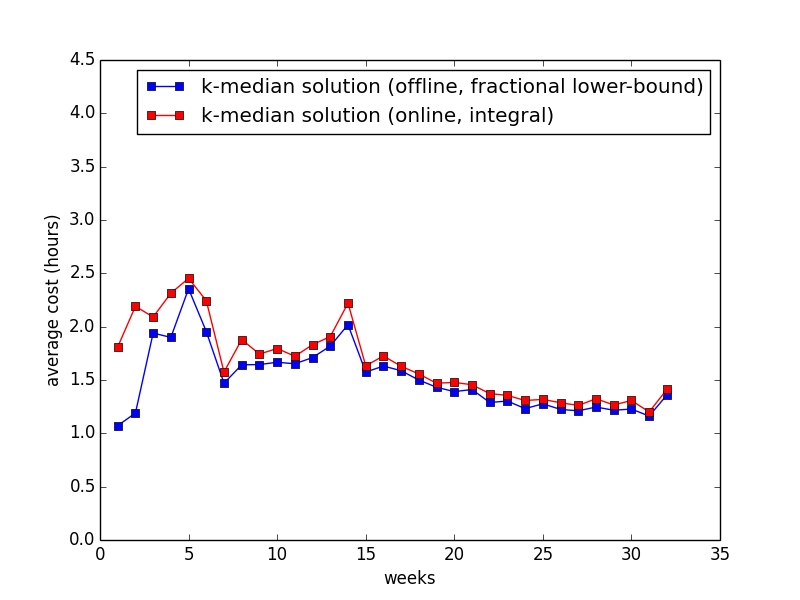
\includegraphics[width=0.30\textwidth]{figs/plot_kmed_CAP100.png}
%%%%%    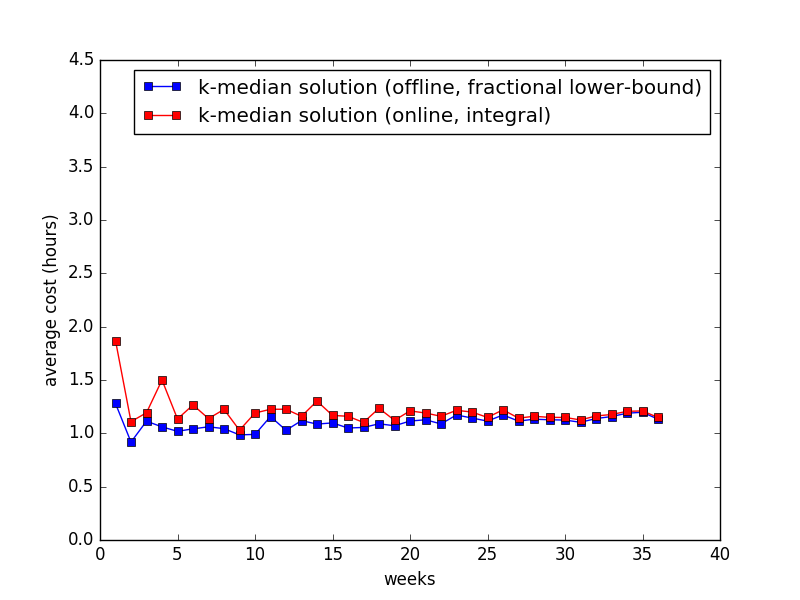
\includegraphics[width=0.30\textwidth]{figs/plot_kmed_CAP100_SL.png}
%%%%%    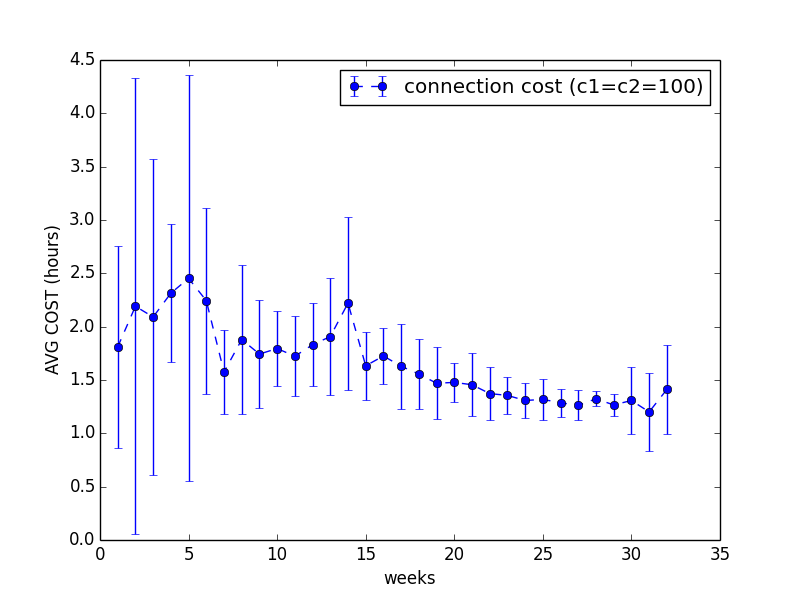
\includegraphics[width=0.3\textwidth]{figs/plot_online_cap100.png}
%%%%%    \caption{Comparing the static and incremental strategies for
%%%%%$s=1$, $w=2$, $k=5, k' = 2$, $cap_1 = cap_2 = 100$ for
%%%%%(a) Liberia, and (b) Sierra Leone.
%%%%%The variance in the solution costs over multiple iterations is shown in (c).}
%%%%%\label{fig:online1}
%%%%%\end{figure}
%%%%%
%%%%%\begin{figure}[h]
%%%%%  \centering % left bottom right top
%%%%%    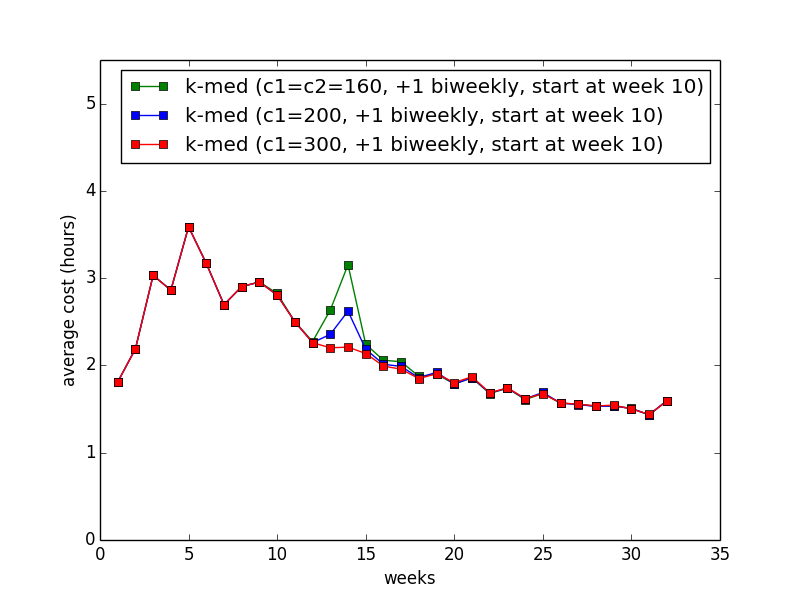
\includegraphics[width=0.45\textwidth]{figs/plot_kmed_c1.png}
%%%%%    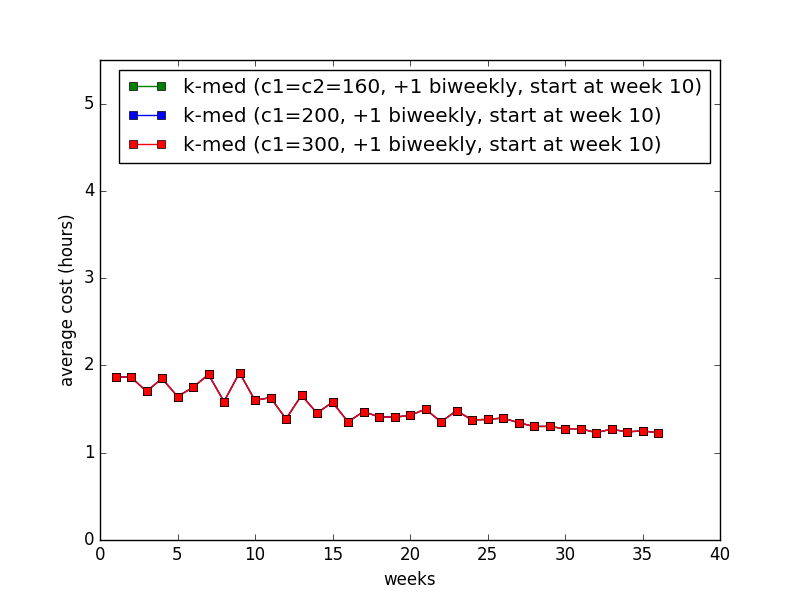
\includegraphics[width=0.45\textwidth]{figs/plot_kmed_c1c2_SL.png}
%%%%%    \caption{Effect of the initial capacity $cap_1$ on the incremental solution, with
%%%%%parameters $s = 10, w = 2, k' = 1, cap_2 = 160$, for (a) Liberia, and (b) Sierra Leone.}
%%%%%\label{fig:online2}
%%%%%\end{figure}
%%%%%
%%%%%\begin{figure}[h]
%%%%%  \centering % left bottom right top
%%%%%    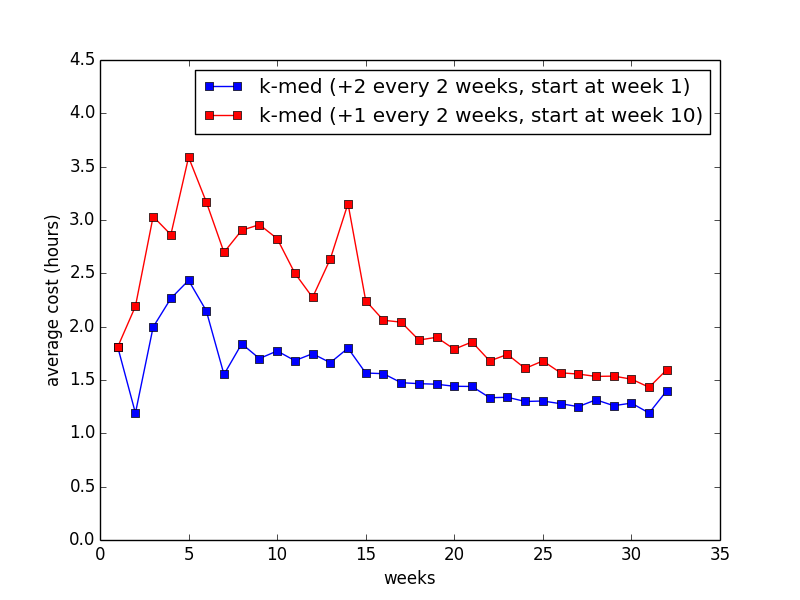
\includegraphics[width=0.45\textwidth]{figs/plot_kmed_CAP160_s1_s10.png}
%%%%%    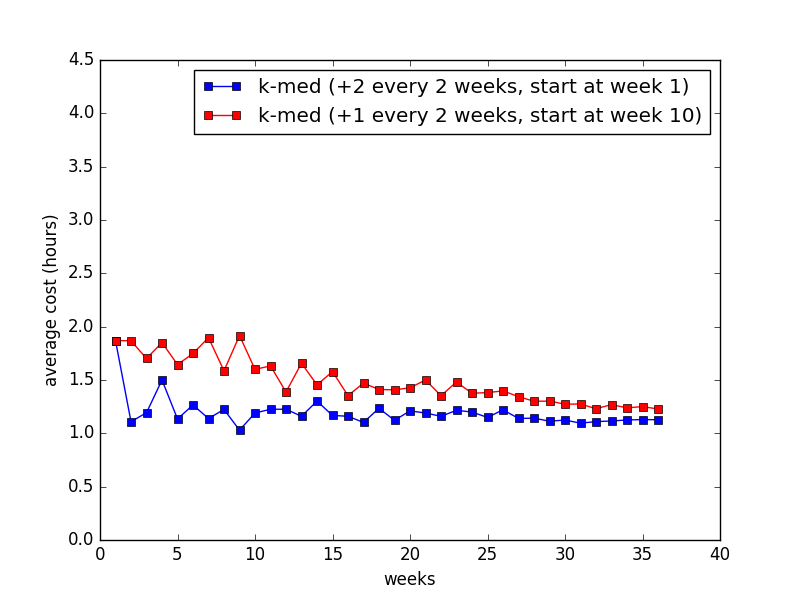
\includegraphics[width=0.45\textwidth]{figs/plot_kmed_CAP160_s1_s10_SL.png}
%%%%%    \caption{Two different opening policies, with kernel size = $5$, for
%%%%%(a) Liberia and (b) Sierra Leone.}
%%%%%\label{fig:online3}
%%%%%\end{figure}
%%%%%
%%%%%
